\documentclass{scrreprt}
\usepackage{listings}
\usepackage{underscore}
\usepackage{graphicx}
\usepackage[bookmarks=true]{hyperref}
\usepackage[utf8]{inputenc}
\usepackage[german]{babel}
\hypersetup{
    bookmarks=false,    % show bookmarks bar?
    pdftitle={Software Architecture Description},    % title
    pdfauthor={Tobias Fischer, Miklós Libak, Eva Norkunas, Lucas Weinknecht}, % author
    pdfsubject={TeX and LaTeX},                        % subject of the document
    pdfkeywords={TeX, LaTeX, graphics, images}, % list of keywords
    colorlinks=true,       % false: boxed links; true: colored links
    linkcolor=blue,       % color of internal links
    citecolor=black,       % color of links to bibliography
    filecolor=black,        % color of file links
    urlcolor=purple,        % color of external links
    linktoc=page            % only page is linked
}%
\def\myversion{0.1 }
\date{}
%\title
\usepackage{hyperref}

\newcommand{\lstinlinejava}[1]{\lstinline[language=java]{#1}}
\newcommand{\lstj}[1]{\lstinlinejava{#1}}

\usepackage{color}

\definecolor{pblue}{rgb}{0.13,0.13,0.7}
\definecolor{pgreen}{rgb}{0,0.5,0}
\definecolor{pred}{rgb}{0.9,0,0}
\definecolor{pgrey}{rgb}{0.46,0.45,0.48}

\lstset{language=Java,
  showspaces=false,
  showtabs=false,
  breaklines=true,
  showstringspaces=false,
  breakatwhitespace=true,
  commentstyle=\color{pgreen},
  keywordstyle=\color{pblue},
  stringstyle=\color{pred},
  basicstyle=\ttfamily,
  moredelim=[il][\textcolor{pgrey}]{$$},
  moredelim=[is][\textcolor{pgrey}]{\%\%}{\%\%}
}

\begin{document}

\begin{flushright}
    \rule{16cm}{5pt}\vskip1cm
    \begin{bfseries}
        \Huge{SOFTWARE ARCHITECTURE DESCRIPTION}\\
        \vspace{1.5cm}
        for\\
        \vspace{1.5cm}
        MELT Chess\\
        \vspace{1.5cm}
        \LARGE{Version \myversion}\\
        \vspace{1.5cm}
        \vspace{1.5cm}
        \today\\
    \end{bfseries}
\end{flushright}

\tableofcontents

\chapter{Einführung}

Die Applikation MELT-Chess unterteilt sich in die Module
\begin{itemize}
\item
  \lstinlinejava{model}: für die Implementierung der Datenstrukturen und Schachregeln
\item
  \lstinlinejava{cli}: für die Implementierung der rudimentären Konsolenschnittstelle mit eingeschränktem Umfang der Features\footnote{Siehe Anforderungen.pdf Dokument}.
\item
  \lstinlinejava{gui}: für die Implementierung der grafischen 2d-Schnittstelle.
\item
  \lstinlinejava{engine}: für die Implementierung der simplen Schach Engine
\end{itemize}

Im Folgenden wird nun der Aufbau dieser vier Module erläutert.

\chapter{\lstj{model}}

Das \lstj{model} Paket teilt sich im wesentlichen in zwei Arten von Klassen: Zum einen die Datenstrukturen \lstj{Piece, Move, Board} und die Implementierung der Schach-Regeln\footnote{gemäß den FIDE-Regeln von 2018} in den Klassen \lstj{MoveGenerator und MoveValidator}. Die Klasse \lstj{Game} verpackt obige Klassen noch einmal für den einfachen Zugriff durch die Clients.

\section{\lstj{Piece}}
Eine Figur wird vollständig durch einen Integer Wert beschrieben, der sich aus $Typ + Farbe$ zusammensetzt. Dazu sind in der Klasse \lstinlinejava{Piece} folgende konstante Felder definiert:

\begin{center}
\begin{tabular}{|l|c|}
  Typ  & Wert \\
  \hline
  None       & 0 \\
  King       & 1 \\
  Pawn       & 2\\
  Knight     & 3\\
  Bishop     & 4\\
  Rook       & 5\\
  Queen      & 6\\
  White      & 8\\
  Black      & 16\\
\end{tabular}
\end{center}

Weiter bietet die Klasse ein paar statische Helfermethoden, eine komplette Auflistung befindet sich in der Java Documentation.

Das Erweitern um mögliche neue Spielfiguren ist ``etwas umständlich'', da die Flags mit Hinblick auf eine Implementierung durch \lstj{byte} anstelle von \lstj{int} geplant wurden. Soll mehr als eine neue Figur eingeführt werden, müssen daher die Flags für die Farben sowie die entsprechenden Bitmasken angepasst werden.


\section{\lstj{Move}}

Die Klasse \lstj{Move} ist eine simple Kapselung für die drei Felder:\newline \lstj{Move(int startSquare, int targetSquare, int flag)},\newline wobei der \lstj{flag}-Parameter optional ist. Für einen Zug sind folgende mögliche Flags definiert:

\begin{center}
\begin{tabular}{|l|c|}
  Typ  & Wert \\
  \hline
  None & 0 \\
  EnPassantCapture & 1\\
  Castling & 2\\
  PromoteToQueen & 3\\
  PromoteToKnight & 4\\
  PromoteToRook & 5\\
  PromoteToBishop & 6\\
  PawnTwoForward & 7\\
\end{tabular}
\end{center}
  


\section{\lstj{Board}}

Die Klasse \lstinlinejava{Board} liefert eine vollständige Beschreibung einer Position auf dem Schachbrett. Dies ist notwendig damit Instanzen von \lstj{Board} dem Spielverlauf hinzugefügt, und somit die Funktionalität ``Rückgängig machen'' implementiert werden kann.

\lstinlinejava{Board} merkt sich die Spielfiguren in einem \lstinlinejava{int[64]} Array, sowie in einer \lstinlinejava{List<Integer>} für die geschlagenen Figuren.

Eine wichtige Methode ist \lstj{Board.makeMove(Move move)}, welche eine neue Instanz von \lstj{Board} zurückgibt in der \lstj{move} ausgeführt wurde. Die Methode beachtet dabei keine der Schachregeln, setzt allerdings beim Bewegen von Figuren die an der Rochade-Regel teilnehmen (also die vier Türme sowie beide Könige) ein entsprechendes Flag das die Rochade verhindert\footnote{Damit wird jedoch keine Regel umgesetzt, die Flags dienen lediglich zum frühzeitigen Abbrechen bei der Generierung von Zügen}.


\section{\lstj{Coordinate}}
Die statische Klasse \lstj{Coordinate} liefert einfache Wege um die verschiedenen Repräsentationen von Brettpositionen (zB ``b7'' $\leftrightarrow$ 9 $\leftrightarrow$ \{1, 1\}) zu konvertieren.


\section{\lstj{MoveGenerator}}
Die \lstj{MoveGenerator} Klasse mit den statischen Auslagerungen implementieren die Regeln zum Bewegen \emph{und nur zum Bewegen} einer Figur\footnote{Das Bedeutet der \lstj{MoveGenerator} liefert auch regelwidrige Züge!}.

Von außen betrachtet sind zwei Methoden interessant:
\newline
\lstj{List<Move> generateMoves()}
\newline
gibt alle möglichen Züge zu gegebener Spielposition zurück.
\newline
\lstj{List<Move> generateMovesStartingAt(int position)}
\newline
gibt alle möglichen Züge zu gegebener Spielposition zurück, die vom Feld \lstj{position} ausgehen.

Für den Fall dass sich die Anforderungen an die Regeln zum Bewegen von Schachfiguren ändern, muss ledliglich von einer dieser Klasse geerbt und gewünschte Regeln überschrieben werden.


\section{\lstj{MoveValidator}}
Der \lstj{MoveValidator} ist eine rein statische Klasse, die zu gegebener Spielposition und einem Zug überprüft ob der Zug Regelkonform ist. Da die Bewegungsregeln bereits in \lstj{MoveGenerator} implementiert sind, wird zunächst überprüft ob der Zug von ihm gefunden wurde. Danach werden noch die folgenden Regeln überprüft:

\begin{itemize}
\item
  Der König steht nach ausführen des Zugs nicht im Schach
  
\item
  Falls der Zug eine Rochade ist, überprüfe das keines der betroffenen Felder angegriffen wird.
  
\item
  Ist der König im Schach und es existiert kein valider Zug nachdem der König nicht mehr im Schach steht, ist das Spiel verloren: SCHACHMATT!
  
\item
  Falls kein valider Zug möglich ist, gibt es ein remis: PATT!\footnote{Laut FIDE-Regeln gibt es noch weitere Möglichkeiten ein remis zu generieren, diese sind aber nicht Teil der Anforderungen.}
\end{itemize}



\section{\lstj{Game}}

Die Klasse \lstj{Game} bietet ein einfaches, übersichtliches Interface zum ausführen eines Zugs und dem erhalten von Informationen der aktuellen Partie für die Clients.




\chapter{\lstj{cli}}


\chapter{\lstj{gui}}
Dieses Aktivitäts Diagramm zeigt (in abstrahiert), wie ein Klick des Users auf dem Spielfeld verarbeitet wird.
Dabei ist zu sehen, dass es nicht für jeden Spielmodus einen eigenen "loop" gibt.
Stattdessen teilen sich die Spielmodi weitgehend funktionen. Dadurch werden Codeduplikate vermieden.

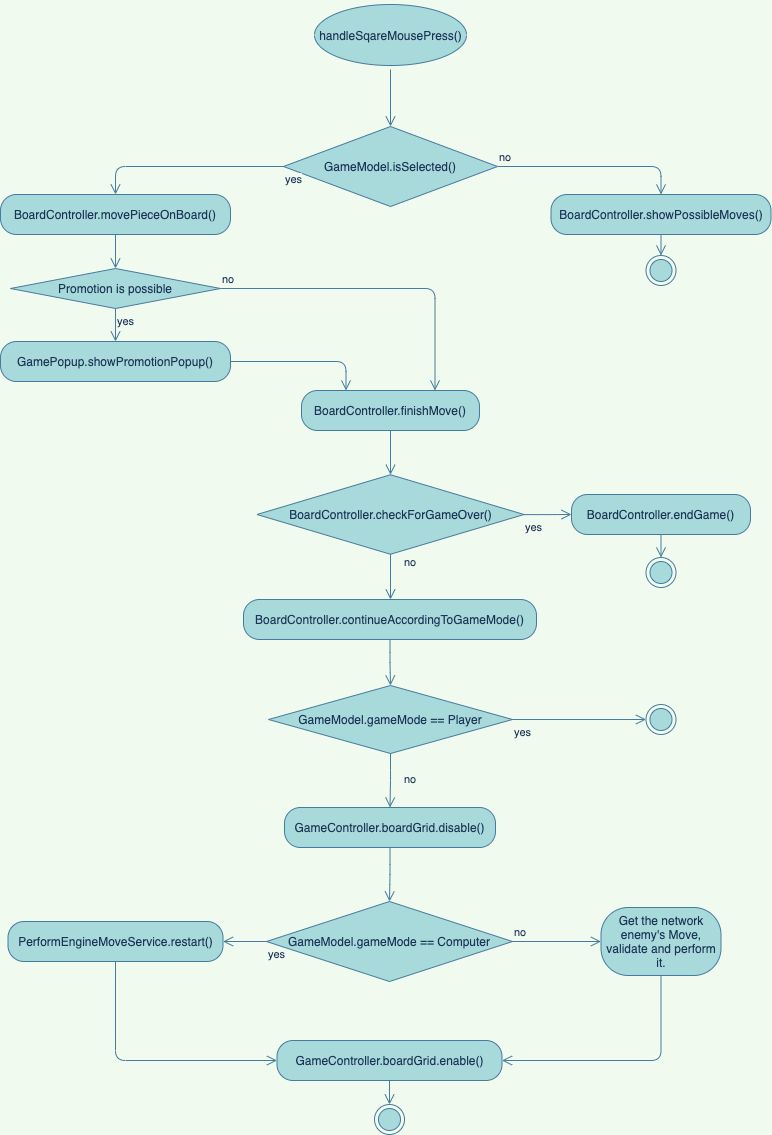
\includegraphics[width=\linewidth]{ActivityDiagramMove}

\chapter{\lstj{engine}}
Die Klasse \lstj{Engine} stellt den Einstiegspunkt zum \lstj{engine} Paket dar und bietet mit \lstj{generateBestMove(Board board)} eine einfache Methode zum generieren neuer Züge an. Des weiter befindet sich im Paket die Klasse \lstj{EngineBoard} welche die Klasse \lstj{Board} aus dem Paket \lstj{model} Erweitert und eine Bewertung der Position ermöglicht. Dies erfolgt mithilfe des \lstj{ScoreGenerator}, in welchem der Materialwert geschlagener Figuren, sowie eine Bewertung für die Position für jede Figur hartkodiert ist. Die Bewertung einer Position ergibt sich durch die aufsummierung dieser einzelnen Werte. Um den bestmöglichen Zug zu finden wird der \lstj{minimax}-Algorithmus angewandt, der durch $\alpha$-$\beta$-pruning beschläunigt wird.

\end{document}
